\subsection{General Overview On Machine Learning}
\label{sub:GeneralML}
This section serves as a summary of general machine learning concepts
which are recommended to better understand the rest of the report.
The theory originates mainly from the machine learning course\cite{learningfromdata2012course} and the accompanying text book\cite{learningfromdata2012book}.

\subsubsection{Types of Machine Learning}
\label{ssub:TypesofMachineLearning}
As mentioned in the \nameref{sec:Introduction} (see Section~\ref{sec:Introduction}),
machine learning is a way of picking a fitting set of data to train on and calculate a model, 
such that similar data can be evaluated using the same model with high accuracy.
Generally speaking there are three popular types of machine learning:
supervised learning, reinforcement learning and unsupervised learning.
The type of learning is often for a project is often chosen on different sets criteria such as the type of data available,
and the knowledge about how the data is grouped.
More often than not the choice will lie on one single solution, something which will become clear in the following paragraphs.

\paragraph{Supervised Learning}
\label{par:SupervisedLearning}
To use supervised learning, the sample dataset used for learning must not only contain some valid input, but also the corresponding ``correct'' output.
The challenge therefore primarily lies on finding the right way of grouping or evaluating the input
such that the corresponding desired output can be achieved, by calculation on the model.
In many ways, this often makes Supervised Learning the most desired method, as there it is often easier to find a fitting solution which corresponds to what is observed on real-world data,
than when the desired output is completely unknown. It is also why, supervised learning has the most different techniques such as linear classification and support vector machines (see Section~\ref{ssub:ModelsforClassification}).

\paragraph{Reinforcement Learning}
\label{par:ReinforcementLearning}
Reinforcement learning is in many ways similar to supervised learning in that it requires both input data and corresponding output to be used.
The main difference is that while supervised learning requires the desired output to be correct, reinforcement only requires a grading of such output.
This technique is therefore often used, when there is no holistic overview regarding the distribution of data but where machine learning is till required.
\begin{exm}
Imagine a hospital where data is gathered on persons with an epidemical illness with multiple stages, and the
medical personnel would want to determine what factors could be causing such illness. As symptoms often can be misinterpreted on early stages,
it is unknown if the outcome is entirely correct but a grading of how ill a patient is can be used to aid the algorithm.
\end{exm}
In many ways reinforcement learning, also has to handle the grading additionally to finding a fitting model. 
This usually makes the models more complex, and as such harder to generalize properly\cite{sutton96generalizationin}\cite{boyan95generalizationin}.

\paragraph{Unsupervised Learning}
\label{par:UnsupervisedLearning}
The last popular type of learning is unsupervised learning, where only data input is given.
In many ways unsupervised learning tries to find a natural grouping or clustering of data,
such that input data that lies next to each other is grouped similarly.
This can be useful to e.g. separate colours from images or to find patterns in given input for further post-processing.
While it maybe hard to find real-world data that groups in obvious ways, and even harder making it fit some desired output;
Unsupervised learning has one advantage, that generalization is free. This is because unsupervised relies solely on input-processing and does not change
any output metrics and as such the models that can be used to not have to conform to an output specification.
Examples of unsupervised learning methods are k-means clustering\cite{learningfromdata2012book}, nearest neighbours\cite{scikitlearn2012nearestneighbours} and PCA\cite{smith2002tutorial}(see Section~\ref{sub:PCA} - \nameref{sub:PCA} for further explanation).

\paragraph{Selected Types of Learning}
\label{par:SelectedTypesofLearning}
To reduce the input space in our project, we resort to the use of PCA, which is as previously mentioned an unsupervised learning technique
and thus have no generalization cost. This allows us both to visualize how the variation/data is grouped, and allows us to
use supervised learning techniques to do the actual separation of data with much less noise and more performance than otherwise.
The choice of supervised learning is due to the fact that it offers the best trade-off between usefulness of output and generalization cost.

\subsubsection{Models for Classification}
\label{ssub:ModelsforClassification}
To be able to classify the resulting data from our experiments, we have chosen some simple supervised machine learning models to apply.
In the following sections we will thus present an overview of these models.
\paragraph{Linear Classification}
\label{par:LinearClassification}
The simplest type of classification is called linear classification.
The idea is simple: given an input dataset $\mathbf{X}$ consisting of data-vectors $\mathbf{x}$ with input parameters $x_1, \dots, x_n \in \mathbf{x}$ and the corresponding output parameter $y \in \left\{-1;+1\right\}$ (see Figure~\ref{fig:linearclass}), 
find a linear formula which separates the outputs given the input parameters.
The classes of output are usually denoted as either being negative (the output being $-1$) or positive (the output being $+1$). 
This makes it easier to run algorithms and is usually not a problem, because it is often possible to do a mapping from any given output format.\\
\begin{minipage}{\linewidth}
\centering
\makebox[\linewidth] {
  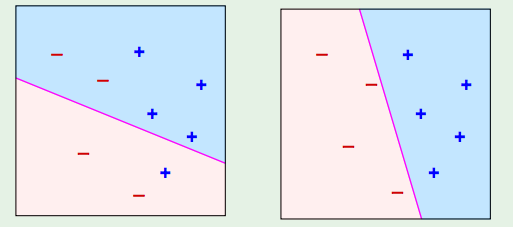
\includegraphics[width=0.5\textwidth]{LinearClassification.png}
}
\captionof{figure}{Linear classification algorithm running on two dimensional linear separable data}\label{fig:linearclass}
\end{minipage}
To separate the two classes of output, a given linear learning algorithm must assign weight coefficients to each input parameter.
To get a positive or negative classification out of the real-numbered output, the sign of the output is taken yielding two output classes.
The equation to be calculated therefore looks as follows:
$$ h(x) = sign(w_0 + w_1 \cdot x_1 + \dots + w_n \cdot x_n ) $$
In order to allow separation of threshold-values that are non-zero an additional learning parameter $w_0$ is added.

\paragraph{Logistic Regression}
\label{par:LogisticRegression}
\paragraph{Support Vector Machines}
\label{par:SupportVectorMachines}
\paragraph{Multiclass Classification}
\label{par:MulticlassClassification}
\subsubsection{Generalization}
\label{ssub:Generalization}
\subsubsection{Error and Noise}
\label{ssub:ErrorandNoise}
\subsubsection{Validation and Testing}
\label{ssub:ValidationandTesting}
